\documentclass[review]{elsarticle}

%GRAPHICS
\usepackage[caption=false,font=footnotesize,margin=10pt]{subfig}
\graphicspath{{Figures/}}
\DeclareGraphicsExtensions{.pdf,.jpg,.jpeg,.png}
\usepackage{color,soul}

%MATH
\usepackage{amsmath}
\usepackage{amssymb}
\usepackage{braket}
\usepackage{enumitem}

%TABLE
\usepackage{array}
\usepackage{multirow}
\usepackage{hhline}

%PDF, URL AND HYPERLINK PACKAGES
\usepackage{lineno}
\usepackage{hyperref}
\makeatletter
\def\url@leostyle{%
  \@ifundefined{selectfont}{\def\UrlFont{\sf}}{\def\UrlFont{\small\ttfamily}}}
\makeatother
\urlstyle{leo}

%BIBLIOGRAPHY
\bibliographystyle{elsarticle-num}

%\modulolinenumbers[5]

\journal{Reliability Engineering \& System Safety}

\begin{document}

\begin{frontmatter}

%% TITLE, AUTHORS, AND ADDRESSES
\title{Survivability Evaluation and Importance Analysis for Cyber-Physical Smart Grids}

\author[sandia]{Mark~Woodard}
%\ead{mjw6y7@mst.edu}

\author[romeo]{Koosha~Marashi}
%\ead{koosha@romeopower.com}

\author[s_and_t]{Sahra~Sedigh~Sarvestani\corref{cor1}}
\cortext[cor1]{Corresponding author}
\ead{sedighs@mst.edu}

\author[s_and_t]{Ali~R.~Hurson}
%\ead{hurson@mst.edu}

%SSS - figure out how to make the author list look better

\address[sandia]{Sandia National Laboratories, Albuquerque, NM 87185, USA}
\address[romeo]{Romeo Power Technology, Vernon, CA 90058, USA}
\address[s_and_t]{Missouri University of Science and Technology, Rolla, MO 65409, USA}

\date{Xxx. XX, 2020}

\begin{abstract}
In this paper, we propose metrics and an evaluation method for survivability, which captures the extent of functionality retained by a system after a disruptive event. Our approach can be applied to a system with an arbitrary, but known, topology. We quantify survivability in terms of the extent and rate of degradation of a domain-specific figure-of-merit. The results are used in importance analysis to identify components most frequently involved in system-level failures, as well as components whose failure have the most severe consequences. As a case study, we have analyzed three smart grids, respectively based on the IEEE 14-, 30-, and 57-bus test systems. Using simulation-based fault injection, we evaluate their survivability in the presence of failures resulting from corrupted data, transmission line outages, and loss of power regulators. Two figures of merit were used, namely the customer service index and the average nominal voltage error. Our work provides means for quantifying and predicting the service degradation caused by failure of parts of a cyber-physical smart grid. It also enables efforts to fortify critical systems and mitigate their inevitable failures.
\end{abstract}

%%%Graphical abstract
%\begin{graphicalabstract}
%%\includegraphics{grabs}
%\end{graphicalabstract}
%
%%%Research highlights
%\begin{highlights}
%\item Research highlight 1
%\item Research highlight 2
%\end{highlights}

\begin{keyword}
smart grid \sep
survivability \sep
importance analysis \sep
cyber-physical systems \sep
quantitative evaluation
\end{keyword}

\end{frontmatter}

%\linenumbers

\section{Introduction}\label{sec:intro}
Modern critical infrastructures are large networked cyber-physical systems ({CPSs}), where a physical system is supplemented with computation, networking, and control, in an effort to improve its efficacy, dependability, or other attributes~\cite{RaI10,DeL12}. Examples of modern critical infrastructures include smart grids, intelligent water distribution networks, and intelligent transportation systems.

CPSs are deployed in unpredictable environments, and hence, modeling and analysis of their behavior in response to cyber and physical faults, errors, and attacks is a critical challenge. In contrast to more common dependability metrics, such as reliability and availability, we find \emph{survivability} better-suited for evaluation of critical systems, which are relied upon for continual, if partial, provision of service even after malfunction or failure of one or more components. Survivability is a measure of a system's ability to continually deliver essential services during an undesirable event~\cite{KnS03}. In this paper, we provide an approach for evaluating the survivability of a cyber-physical power grid system and identifying the components most critical to this survivability. In our review of the relevant literature, we identified a research gap between survivability definitions and means of quantifying a system's survivability. Proposed metrics in the existing studies often fail to capture attributes on which a survivable behavior relies. We aim to address this gap by identifying key elements that indicate a survivable behavior and proposing means of calculating a smart grid system's survivability using its abstracted behavior metrics.

Large-scale and cascading failures of critical infrastructures motivate this work. One example occurred in September 2003, where a cascading power failure left half of Italy without power for multiple days~\cite{BeA04}. This failure was exacerbated by the loss of Internet communication nodes left without power, which in turn caused further breakdown of communication and control at multiple power stations. Another example is the Arizona-Southern California blackout in September 2011, which occurred as the result of an 11-minute outage of a 500 kV transmission line. The outage triggered a cascade that left approximately 2.7 million customers without power for several hours~\cite{FERC12}. Although the system was designed to withstand the outage of a single line, the situation was exacerbated by higher than normal demand during peak hours, combined with lower than peak generation. A subsequent study of this blackout~\cite{FERC12} found that inadequate situational awareness contributed to this and many other blackouts. These examples demonstrate the dependence of CPSs on accurate real-time data, especially for failure mitigation. More robust designs are required for prevention of future blackouts, and modeling and simulation tools are needed to rigorously evaluate these designs prior to deployment.

Our approach for evaluation of survivability relies upon identification of a domain-specific \emph{figure-of-merit ({FoM})} that is indicative of the extent to which one or more essential services are being provided by the system. FoM can be defined as soon as fundamental requirements of a system are specified. In the system design phase, a set of plausible failure cases needs to be identified. In this context, a \emph{failure case} is defined as failure of one or more specific components. For each failure case, the FoM is observed to determine the \emph{extent} and \emph{rate} of service degradation that results from the disruption. An overview of a system design verification cycle that utilizes our proposed method of survivability evaluation is outlined below.

\begin{enumerate}
  \item An appropriate FoM and a set of representative failure cases are identified during the initial design phase of the system.
  \item Once the system is implemented, changes in the FoM are observed - in a field, laboratory, or simulation environment - over the duration of each failure case.
  \item Survivability is quantified in terms of the \emph{extent} and \emph{rate} of degradation of the FoM during failures.
  \item Components whose failure is the most detrimental to survivability are identified and hardened.
  \item Steps 2 through 4 are repeated as necessary until desired a level of survivability is attained.
\end{enumerate}

Utilizing FoM provides an abstraction that enables applicability of the approach to a broad range of systems, however, this work studies the application of the proposed technique only in smart grid domain. In a smart grid application, our method provides i) a means for specifying verifiable survivability requirements for the system to be designed and ii) an approach for verifying whether a design meets those requirements. More specific contributions of this work are as follows.

\begin{enumerate}
  \item Identifying and calculating quantitative metrics, derived from service provision indices, that are justifiably attributed to the survivability of smart grid systems.
  \item Proposing a method for analysis of survivability using the extent of functionality retained by a smart grid system after a set of disruptive events.
  \item Introducing and validating a method for identifying components of a system that are most critical to its survivability.
\end{enumerate}

The remainder of this paper is structured as follows. Section~\ref{sec:rel_work} discusses survivability and other non-functional attributes related to dependability and summarizes related literature on modeling of survivability. In Section~\ref{sec:approach}, we describe our approach to survivability evaluation and demonstrate how the survivability metrics can be used to identify components most critical to survivability. In Section~\ref{sec:case_study}, we apply these techniques to three smart grids, respectively based on the IEEE 14-, 30-, and 57-bus test systems. We conclude the paper and outline future extensions to this research in Section~\ref{sec:conc}. All data underlying the work reported in this paper has been made available on our GitHub repository for the project~\cite{dataset}.

\section{Background and Related Work}
\label{sec:rel_work}
Quantitative evaluation of systems (or components) can be based on \emph{functional} or \emph{non-functional} metrics. Non-functional metrics assess the overall system operation, rather than any specific system behavior. \emph{Dependability}, as defined by Avizienis et al.~\cite{AvL04}, characterizes system operation as related to failures and recovery. It describes the behavior of a system over its lifetime---its ability to deliver services and to avoid and recover from faults. Dependability of CPSs, as investigated in~\cite{Er10,HaL10}, encompasses aspects of the ability of the system to withstand failure of both cyber and physical components. While both qualitative~\cite{MoK10,Ri04} and quantitative~\cite{VeS12,FaS09b} models have been proposed, the majority of studies on the dependability of CPSs are qualitative in nature.

Although dependability attributes are well-studied for small-- to large--scale networks and systems, they fall short in describing characteristics of complex CPSs. For example, reliability and availability, two important aspects of dependability, consider the system state to be binary--\emph{operational} or \emph{failed}. This view is inadequate for critical infrastructures, which are expected to deliver uninterrupted service despite continual disturbances. It is expected that a large-scale system will spend time in functionally degraded states, without interruption of \emph{essential services}. Consequently, additional non-functional attributes are required to characterize these degraded, yet operational states.

\emph{Performability}, introduced by Meyer~\cite{Me80}, combines performance and availability to evaluate system effectiveness, taking into account behavior following failures. In other words, a system can be in a fully functional state, a partially operational state with degraded performance, or a failed state. Performability describes the expected performance of a system over a duration composed of alternating functional/degraded/failed periods. As a metric, \emph{resilience} can also be considered a refinement of availability. Resilience is defined as the ability of a system to bounce back from failure~\cite{HeR12,HoB16}. Therefore, its application is limited to the recovery phase that follows a failure.

Introducing performability as a metric that combines availability (pessimistic, binary view of operation) and performance (optimistic, neglects periods of inoperability) is an effort to attain a realistic view of the system. \emph{Survivability} is another non-functional attribute that was introduced with a similar objective, and is used to characterize degraded operation. Survivability, unlike resilience, can be used to describe degraded operation at any point after a disturbance occurs, regardless of whether the disturbance is a fault tolerated by the system, or a failure that actually causes degradation. Critical CPSs, including smart grids, are expected to autonomously defend against attacks, remedy the consequences of failure, and recover in a timely manner. Dependability attributes provide coarse-grained characterization of these qualities, unlike survivability metrics, whose purpose is to precisely characterize transient behavior after a disturbance. For this reason, survivability is used in a wide array of application domains, including weapons systems engineering~\cite{Ba03}, telecommunication services~\cite{STD1037}, information systems~\cite{ElF97}, and software engineering~\cite{DeW88}.

We were unable to infer a ``standard'' definition of survivability in the literature; perspectives on the topic are diverse~\cite{AvC15}. A qualitative and concise definition is presented by Heegaard and Trivedi~\cite{HeT09}:
\begin{quote}
``Survivability is the system's ability to continuously deliver services in compliance with the given requirements in the presence of failures and other undesired events.''
\end{quote}

ANSI T1A1.2 working group~\cite{T1A1} identifies parameters of an FoM that are associated with survivable behavior of a system. To better illustrate the differences between the aforementioned dependability-related attributes, one operation and recovery cycle of a repairable system is shown in \figurename~\ref{fig:fom}. Note that $M(t)$ denotes an FoM chosen to represent the behavior or performance of the system over time.

\begin{figure}[!ht]
\centering
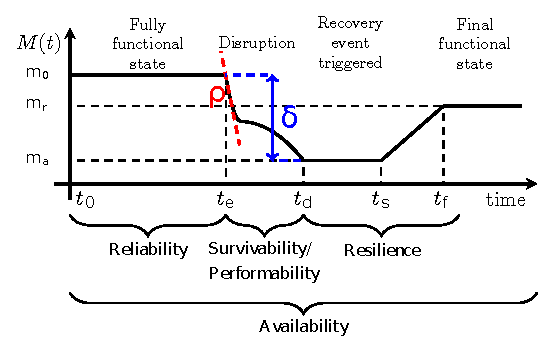
\includegraphics[width=.9\columnwidth]{fom}
\caption{Durations of applicability for dependability-related metrics.}
\label{fig:fom}
\end{figure}

Comparison of survivability evaluation techniques is complicated by the lack of a common definition for this attribute. Knight et al.~\cite{KnS03} present a survivability definition and model based on a service state-transition graph constructed from a six-tuple of service specification levels, service value factors, reachable environmental states, relative service values, set of valid transitions, and service probabilities. Ma~\cite{Ma12} similarly quantifies survivability as a four-tuple of resistance, resilience, persistence, and failure count. In~\cite{Ma12}, \emph{resistance} is described as the ability to withstand an attack, \emph{resilience} refers to the mean recovery time from a catastrophic failure, \emph{persistence} is the ability to maintain or exceed the minimal threshold of required functionality, and \emph{failure count} describes the number of failures encountered over the duration of observation. These individual attributes are well-defined, but not in a unified fashion, and hence, the study does not lead to a practical approach for quantitative evaluation of survivability.

In traditional power grids, reliability and availability metrics, such as system average interruption duration index (SAIDI), were adequate for characterization of dependability. The richer feature set typical of a smart grid motivates the use of more refined metrics, such as survivability. Menasch{\'e} et al.~\cite{MeM12} have proposed an enhancement to the SAIDI metric. Their measure is denoted as \emph{ESAIDI} and applied to evaluation of survivability aspects of a smart grid. ESAIDI is intended to facilitate analysis of the consequences of failures in distribution automation in the power grid. Avritzer et al.~\cite{AvS13} utilize the same approach and further extend the model to account for disruptions in the communication infrastructure. This work was later combined with power flow analysis to create a survivability model that facilitates optimal design for the automation system of a smart grid~\cite{KoA13}. A subsequent extension of the work~\cite{MeA14} allowed for concurrent failures in the power system. All of these approaches~\cite{MeM12,AvS13,KoA13,MeA14} use time-to-recovery as a measure of survivability. However, time-to-recovery spans both the failure and recovery processes, and hence, cannot be used to separately evaluate system during each of these two phases.

Chopade and Bikdash~\cite{ChB12} present a model for survivability of a smart grid, based on graph-theoretic measures such as degree distribution and clustering coefficient. All buses (vertices) and lines (edges) are assumed to be identical. This is an unrealistic assumption given that reliability and other attributes of buses and lines can vary significantly in a power grid. In a similar vein, \cite{YiD15} evaluates the survivability of mobile ad hoc networks (MANETs) as the probability that all active nodes are $k$-connected to the network. This probability is determined using a semi-Markov model that captures state transitions due to node failures and malicious attacks. The connectedness of MANETs is a representative measure of their functionality; thus, the probability of being $k$-connected can reflect survivability. The proposed method is ill-suited for evaluation of any system expected to provide services beyond connectivity.

Avritzer et al.~\cite{AvC15} survey recent approaches to survivability evaluation of water, gas, and electricity infrastructures. Stochastic hybrid models such as fluid stochastic Petri nets, hybrid Petri nets, and piece-wise deterministic Markov processes, as well as graph-theoretic approaches, are among the methods described.

Table~\ref{tab:related_work} compares our proposed method to the aforementioned approaches. The distinction of our work as compared to the closest study~\cite{ChB12} is its higher resolution in defining system state space as well as its potential for broad applicability to a range of domains - the FoM reflects domain-specific aspects of the system's operation, but the survivability evaluation based on this FoM is general. In other words, the definition of FoM provides an abstraction of the system behavior that enables the use of a generic method for detecting survivable behaviors. This breadth facilitates analysis of CPSs, where features such as complexity and heterogeneity render other methods inapplicable.

\begin{table*}[!ht]
\caption{Comparison of survivability evaluation techniques described in Section \ref{sec:rel_work}.}
\label{tab:related_work}
\renewcommand{\arraystretch}{1.1}
\newcommand{\mcline}{\cline{2-3} \cline{4-5} \cline{6-6} \cline{7-7} \cline{8-9}}
\newcommand{\mr}[1]{\multirow{2}{*}{#1}}
\newcommand{\mc}[1]{\multicolumn{2}{c}{#1}}
\newcommand{\mcl}[1]{\multicolumn{2}{c|}{#1}}
\newcommand{\Qualitative}{\rotatebox{270}{Qualitative}}
\newcommand{\Quantitative}{\rotatebox{270}{Quantitative}}
\newcommand{\Known}{\rotatebox{270}{Known}}
\newcommand{\Random}{\rotatebox{270}{Random}}
\centering
\begin{tabular}{@{\extracolsep{4pt}}|c|cccccccc|} \hline
\mr{Reference}&     \mc{Definition}      &      \mc{Modeling}       &Evaluation&Simulation&\mcl{System Topology} \\ \mcline
              &\Qualitative&\Quantitative&\Qualitative&\Quantitative&          &          &\Known    &\Random    \\[6em] \hline
\cite{KnS03}  &\checkmark  &             &            &             &          &          &          &           \\
\cite{AvC15}  &            &             &            &             &\checkmark&          &\checkmark&\checkmark \\
\cite{HeT09}  &            &             &\checkmark  &\checkmark   &\checkmark&\checkmark&\checkmark&           \\
\cite{Ma12}   &            &\checkmark   &            &             &          &          &          &           \\
\cite{MeM12}  &            &             &            &\checkmark   &\checkmark&          &\checkmark&           \\
\cite{AvS13}  &            &             &            &\checkmark   &\checkmark&          &\checkmark&           \\
\cite{KoA13}  &            &             &            &\checkmark   &\checkmark&          &\checkmark&           \\
\cite{MeA14}  &            &             &            &\checkmark   &\checkmark&          &\checkmark&           \\
\cite{ChB12}  &            &             &            &\checkmark   &\checkmark&\checkmark&          &\checkmark \\
\cite{YiD15}  &            &             &            &\checkmark   &\checkmark&\checkmark&          &\checkmark \\
This paper    &            &             &            &\checkmark   &\checkmark&\checkmark&\checkmark&           \\ \hline
\end{tabular}
\end{table*}

\section{Proposed Approach}
\label{sec:approach}
For many systems, including critical infrastructures, the high availability required makes it infeasible to bring down the system for fault injection studies. Detailed reports of real-world failures are few and far between, and many possible failure scenarios have never actually occurred in practice, necessitating the use of simulation tools. No simulation environment perfectly captures the characteristics of real-world entities; however, simulation does provide a good understanding of system behavior at minimal cost. Our goal is to enable survivability evaluation for smart grids with cyber-physical complexities, with an approach that can utilize data from simulation, laboratory and/or field observation, and/or historical data about failures of a system.

\subsection{Survivability Attributes}
\label{sec:approach:attr}
In~\cite{HeT09}, \emph{graceful degradation} and \emph{failure resistance} are mentioned as two attributes essential to survivability. In defining metrics for survivability, we describe these attributes (with reference to \figurename~\ref{fig:fom}) as follows:

\begin{itemize}[leftmargin = *]
    \item \emph{Graceful degradation} is achieved when the \emph{rate of degradation}, $\Big|\dfrac{dM(t)}{dt}\Big|$, after a disturbance is considered to be slow, in the context of the time scale of the system domain.
    \item \emph{Failure resistance} indicates that the \emph{extent of degradation}, $|M(t_d) - M(t_e)|$, resulting from a disturbance, i.e., the loss in FoM value incurred between the start of the disturbance and initiation of recovery, leaves the system functionality at a level considered to be acceptable.
\end{itemize}

The FoM is domain-specific, as it is intended to capture the extent to which a system is delivering essential services. In this paper, we consider the FoM to represent a single service. Our survivability evaluation approach can be used to represent more complex behavior by defining an FoM that is a composite, e.g., a weighted average, of metrics that reflect different essential services.

These two attributes are pivotal to our methods for survivability evaluation and importance analysis, which are described in Sections \ref{sec:approach:eval} and \ref{sec:approach:importance}, respectively.

\subsection{Evaluation of Survivability}
\label{sec:approach:eval}
We evaluate survivability through the following actions, carried out consecutively:
\begin{enumerate}
    \item A system-specific FoM and a set of representative failure cases are selected to evaluate the system.
    \item Each failure case is observed or simulated, and the value of the FoM is monitored over an interval that begins with a fully functional system, includes a disruption that causes degradation to the FoM, and continues through initiation of recovery efforts.
    \item The rate and extent, respectively, of degradation of the FoM are calculated from the log of FoM values.
\end{enumerate}

In this context, a \emph{failure case} denotes the set of distinct components whose failure initiates a specific disturbance to the system. In reality, varying the order and timing of the failures of the same set of components can lead to several different failure cases. In this initial stage of our research, for simplicity and tractability, we assume concurrent failure of all components comprising a failure case. Therefore, we can represent failure case $j$, denoted as $\mathbf{F}_j$, as the set of components whose concurrent failure (at time $t_e$ in \figurename~\ref{fig:fom}) has initiated the disturbance being examined. In contrast to system-level operation, which we represent by an FoM that can take any of a range of values, we consider component-level operation to be binary, i.e., a component is either fully functional or has failed altogether. This assumption is justified where the system representation is fine-grained to the extent that the contribution of a single component to delivery of an essential service cannot be further decomposed.

Exhaustive examination of failure cases is infeasible for large complex systems. On the other hand, the omission of failure cases with catastrophic consequences could render survivability evaluation meaningless. Explosion of the state space is a common problem in many types of analysis. It resolution is not within the scope of this paper. Existing literature on software or system testing~\cite{CoR79} can provide inspiration for reducing the size of the state space. In this paper, we will assume a predefined set of failure cases as the basis of survivability evaluation.

Let a system with $n$ components and $m$ failure cases be designated as the basis of survivability evaluation. Each failure case is observed or simulated for a duration that begins with a fully functional system where all components are operational, continues through the disturbance caused by failure of the components in $\mathbf{F}_j$, and ends when recovery efforts are initiated. In other words, observation or simulation of the failure case defined by $\mathbf{F}_j$ produces a record of the FoM, $M_j(t)$, for $t_0 \leq t \leq t_d$, where $t_0$ and $t_d$ are as defined in \figurename~\ref{fig:fom}. The initiating disturbance at $t_e$, $\mathbf{F}_j$, can trigger the failure of other components. We define $\mathbf{C}_j$ as the set of all components whose failure is observed between $t_e$ and $t_d$.

Survivability analysis requires that $M_j(t)$ be examined to determine the extent and rate of degradation. In terms of \figurename~\ref{fig:fom}, we seek to determine the full extent of degradation, denoted as $\delta_j$, incurred between the instant of disturbance,~$t_e$, and initiation of recovery,~$t_d$. Over the same period, the most rapid rate of degradation is denoted as $\rho_j$. Equations \eqref{eqn:extent} and \eqref{eqn:rate}, respectively, describe these attributes. The survivability of a system is determined by aggregating the extent and rate of degradation for all failure cases.

\begin{eqnarray}
\label{eqn:extent}
\delta_j = \max_{t_0 \leq t \leq t_d} |M_j(t_0) - M_j(t)|\\
\label{eqn:rate}
\rho_j = \max_{t_0 \leq t \leq t_d}\Big|\dfrac{dM_j(t)}{dt}\Big|
\end{eqnarray}

Our proposed evaluation technique relies on the assumption that the extent and rate of degradation collectively capture the ability of a system in continually delivering its essential services during disruptions. Therefore, we model the survivability in a two-dimensional Euclidean plane, where the rate of degradation for each failure case is depicted on the horizontal axis and its extent of degradation is depicted on the vertical axis. A given failure case with a rate of degradation of $\rho_j$ and an extent of degradation of $\delta_j$ is illustrated with a degradation point at coordinates $(\rho_j, \delta_j)$. This visualization of the FoM, as shown in \figurename~\ref{fig:degrad_pt}, facilitates evaluation of survivability. We further define the \emph{degradation index} as the Euclidean distance from the degradation point to the origin, as shown in Equation \eqref{eqn:degrad_index}. The definition of degradation index incorporates $\rho$ and $\delta$ proportionately and normalizes the index to a $[0, 1]$ range.

\begin{equation}
\label{eqn:degrad_index}
\phi_j = \sqrt{\rho_j^2 + \delta_j^2}
\end{equation}

An example of a single degradation point for an arbitrary failure case is shown in \figurename~\ref{fig:degrad_pt}, where $\rho = 0.25$, $\delta = 0.6$, and $\phi = 0.65$. The degradation index facilitates comparison of failure cases and can be averaged across all failure cases to calculate a single survivability index for the system.

\begin{figure}[!ht]
\centering
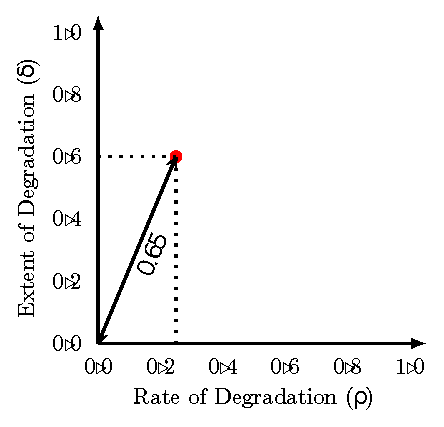
\includegraphics[width=1.85in]{degrad_pt}
\caption{Degradation point ($\rho, \delta$) for a failure case and the resulting degradation index.}
\label{fig:degrad_pt}
\end{figure}

Creating a two-dimensional color intensity histogram of the degradation index, over all failure cases considered, can facilitate identification of clusters indicative of failure cases that are similar in consequence. In an ideal system, only one cluster would be evident, near the origin, in the lower left corner of the plot. This cluster is characterized by slow and minimal degradation of the system. Clusters outside of this area represent failure cases that merit further investigation, as they reflect non-survivable behavior.

\subsection{Importance Analysis}
\label{sec:approach:importance}
Evaluation of survivability can illuminate weaknesses in a system. Specifically, our method can facilitate identification of components most in need of fortification, i.e., \emph{importance analysis}, where the measure of importance is the contribution of a component to survivability. We propose two criteria for ranking components, namely \emph{criticality} and \emph{fragility}.

The criticality of a component is determined by three factors associated with the dynamics of the FoM after its failure: i) overall system degradation, ii) immediate drop of FOM, and iii) immediate change in the rate of degradation. To determine the criticality of the $i^\mathrm{th}$ component, we need to identify every failure case in which it was observed to fail. Let $\mathcal{S}_i = \set{j | i \in \mathbf{C}_j}$ denote this set of failure cases. Equation \eqref{eqn:criticality} shows the calculation of the criticality of component $i$, denoted as $\alpha_i$.
\small
\begin{equation}
\label{eqn:criticality}
\alpha_i =
\frac{1}{m}
\sum\limits_{j \in \mathcal{S}_i}
\left(
\overbrace
  {\dfrac
    {\delta_j}
    {\max\limits_{1 \leq l \leq m} \delta_l}
  }
  ^{\text{first term}}\cdot
\overbrace
  {\dfrac
    {\dfrac{d M_j(t)}{dt}\Big|_{t=t_{i, j}}}
    {\max\limits_{\forall t}\dfrac{d M_j(t)}{dt}}
  }
  ^{\text{second term}}\cdot
\overbrace
  {\dfrac
    {\dfrac{d^2 M_j(t)}{dt^2}\Big|_{t=t_{i, j}}}
    {\max\limits_{\forall t}\dfrac{d^2 M_j(t)}{dt^2}}
  }
  ^{\text{third term}}
\right)
\end{equation}
\normalsize
where $t_{i, j}$ denotes the time at which component $i$ fails during failure case $\mathbf{F}_j$. In Equation \eqref{eqn:criticality}, the three terms capture the factors explained above. Adding the respective products across all failure cases involving component $i$, provides a measure of the total impact of the failure of $i$. Dividing this number by $m$, the total number of failure cases, normalizes the criticality and facilitates comparison of different components.

A less precise measure of the importance of a component is provided by \emph{fragility}, which reflects the fraction of observed or simulated failure cases in which the component has failed. The fragility of component $i$, denoted as $\beta_i$ , can be determined as shown in Equation \eqref{eqn:fragility}, where $m$ is the total number of failure cases.
\begin{eqnarray}
\label{eqn:fragility}
\beta_i = \frac{|\mathcal{S}_i|}{m}
\end{eqnarray}

Either criticality or fragility can be used to determine the priority of a component for hardening efforts. Given that fragility is calculated without consideration of service degradation (as represented by the FoM), its use is recommended only in cases where failure information does not involve the exact time when each component failed.

\section{Case Study: Smart Grids}
\label{sec:case_study}
In this section, we demonstrate our proposed approach by applying it to a number of smart grids based on test systems commonly used in power engineering literature. Specifically, we demonstrate survivability evaluation for smart grids based on the IEEE 14-, IEEE 30-, and IEEE 57-bus test systems~\cite{PSTCA}. The IEEE 14-bus system has been included in the interest of providing a concise and clear example. The two larger systems demonstrate the scalability of our method. All three systems are depicted in \figurename~\ref{fig:ieee_bus_systems}.

\begin{figure*}[!ht]
\centering
\subfloat[IEEE 14-bus smart grid]
{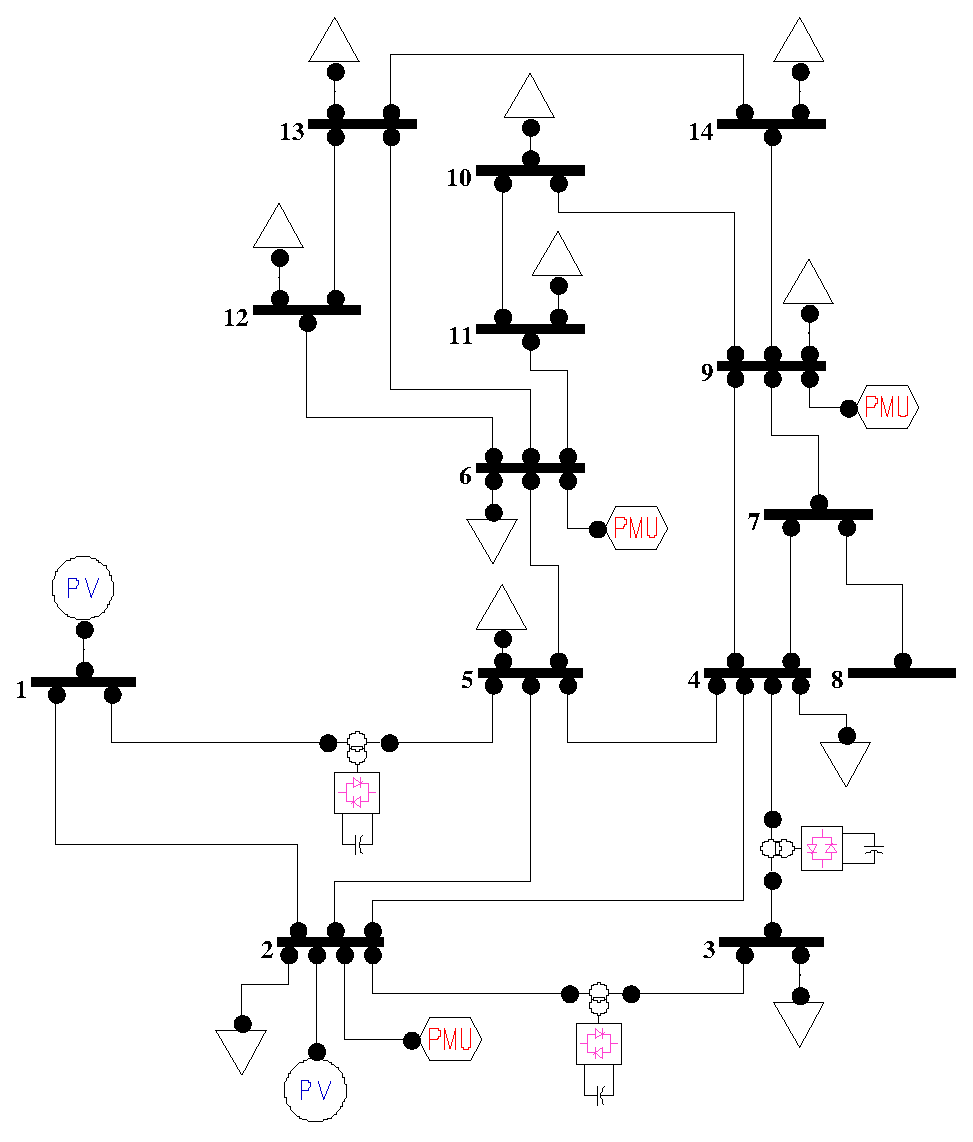
\includegraphics[width=0.33\textwidth]{ieee14}
\label{fig:ieee14}}
~
\subfloat[IEEE 30-bus smart grid]
{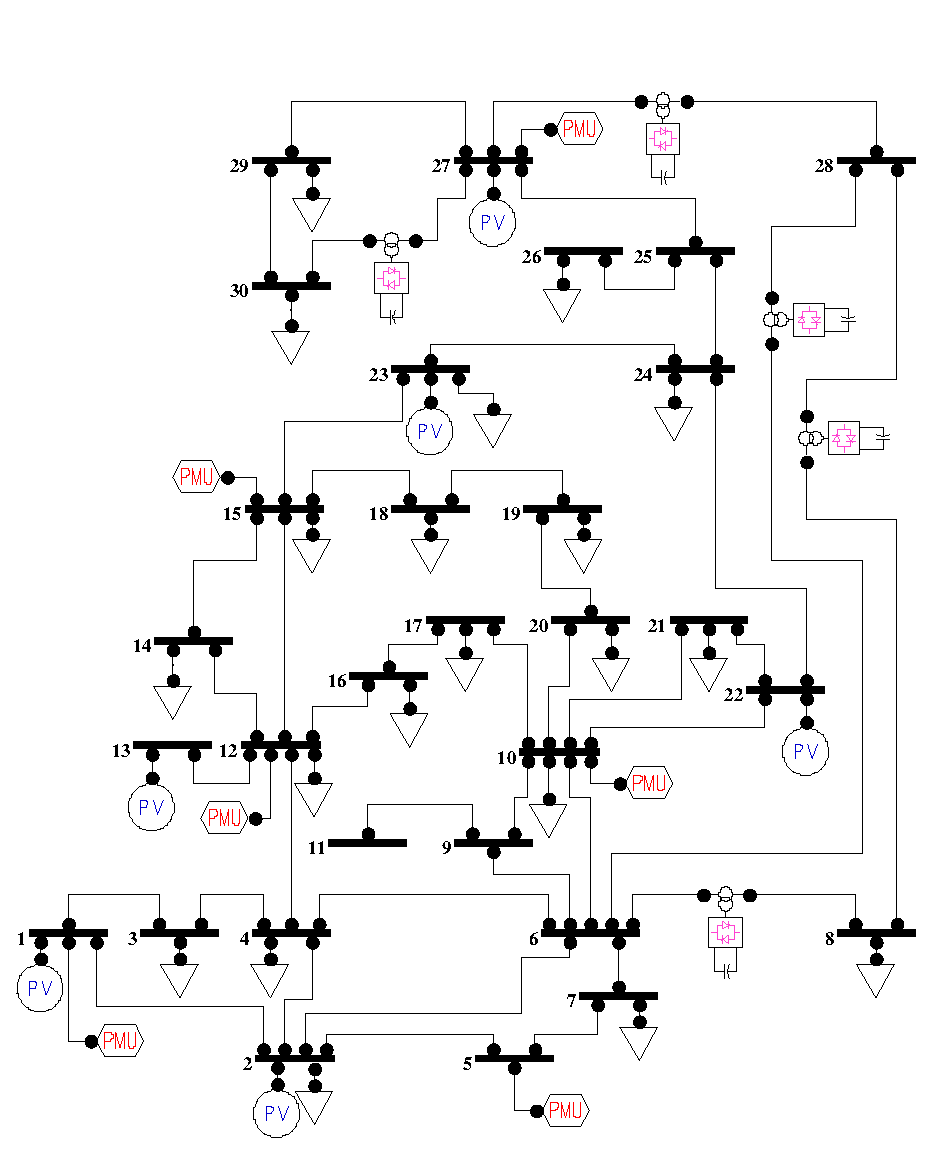
\includegraphics[width=0.38\textwidth]{ieee30}
\label{fig:ieee30}}
\hfil
\subfloat[IEEE 57-bus smart grid]
{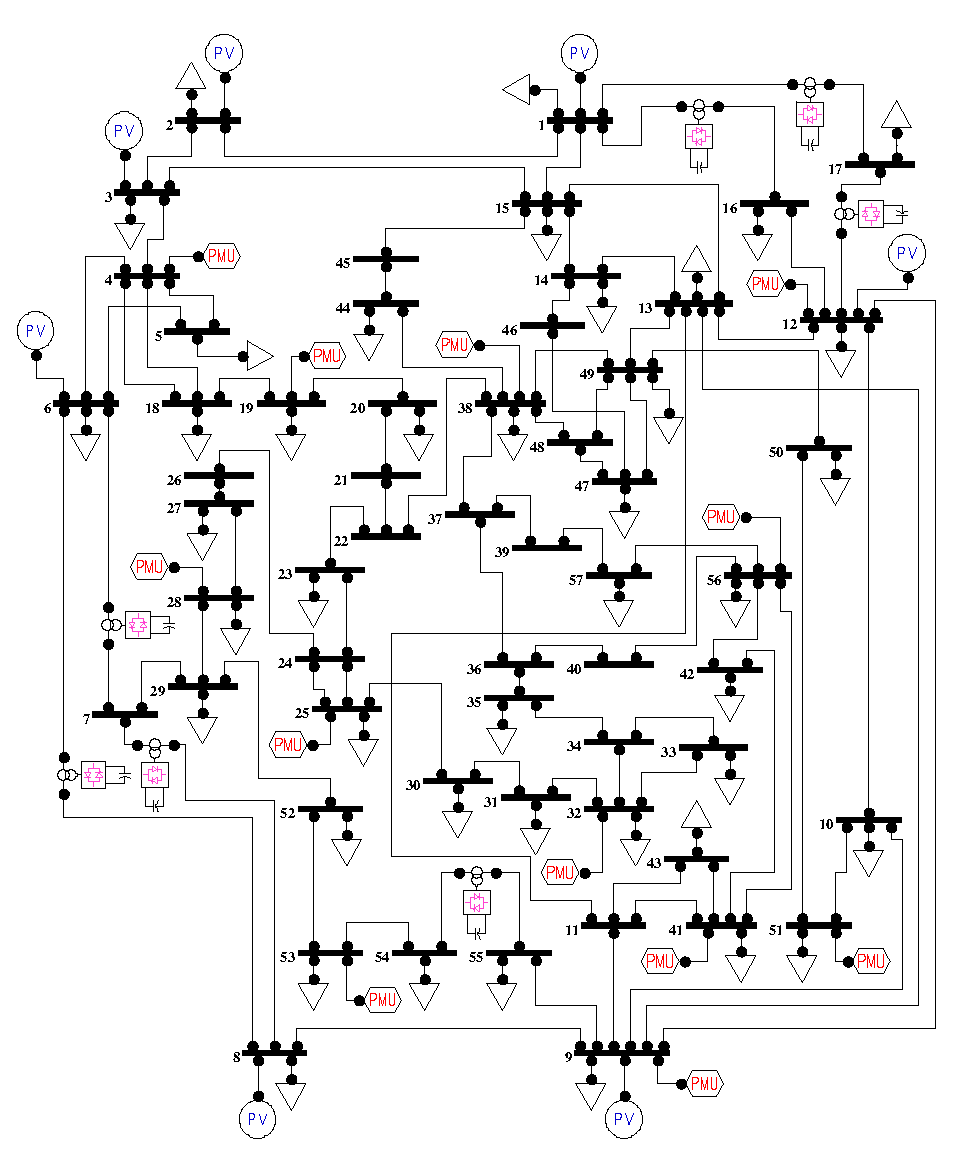
\includegraphics[width=0.50\textwidth]{ieee57}
\label{fig:ieee57}}
~
\subfloat
{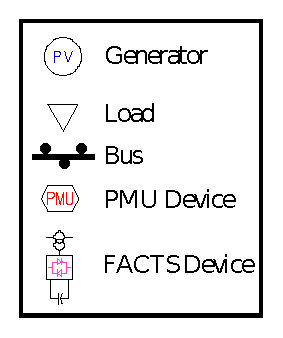
\includegraphics[width=0.15\textwidth]{ieee_cases_legend}
\label{fig:ieee_legend}}
\caption{Single-line diagrams of IEEE smart grid test systems.}
\label{fig:ieee_bus_systems}
\end{figure*}

Our approach to survivability evaluation is intended to be applicable to smart grids with intertwined cyber and physical  components. To demonstrate our approach for this CPS, we supplemented three classic IEEE test systems with cyber infrastructure to create respective smart grids. Our cyber infrastructure comprises phasor measurement units (PMUs), which record and communicate dynamic power system data synchronized using GPS, flexible AC transmission system (FACTS) devices, which adjust the flow of power in transmission lines, and a decision support algorithm that determines optimal settings for the FACTS devices based on data from the PMUs.

\subsection{Selection of the Figure-of-Merit}
\label{sec:case_study:sel_fom}
The \emph{essential service} expected of a smart grid is provision of stable power to customers. We define two FoMs to this end. The first FoM is the \emph{customer service index} (CSI), which reflects the fraction of customers who have received the essential service in question. CSI takes a binary view of service -- a customer has either been provided with adequate power or is not considered to have been served at all. In accordance with standards such as EN-50160~\cite{EN50160}, our determination of whether a customer has been served is based on whether the voltage of the bus to which the customer is connected is within a predetermined range. For example, EN-50160 specifies a range of 0.9 to 1.1 per-unit, where the per-unit representation denotes normalization by a base value, in this case, a base voltage. The CSI is calculated from customer information as in Equation \eqref{eqn:csi}.
\begin{equation}
\label{eqn:csi}
\text{CSI}=\frac{\text{\footnotesize Number of customers served}}{\text{\footnotesize Total number of customers}}
\end{equation}

The second FoM we propose for evaluating smart grid survivability is the \emph{average nominal voltage error} (ANVE), which is calculated from the average voltage error over all load buses that experience under-voltage or over-voltage, as in Equation \eqref{eqn:anve}. An ANVE of 1 indicates that the grid is providing full service. In contrast with CSI, which solely reflects blackouts, ANVE considers brownouts as well.
\begin{equation}
\label{eqn:anve}
\text{ANVE}=1 - \frac{\sum\limits_{i}\left|\text{\footnotesize Rated voltage at bus}\;i - \text{\footnotesize Actual voltage at bus}\;i\right|}{\text{\footnotesize Total number of customers}}
\end{equation}

\subsection{Selection of Failure Cases}
\label{sec:case_study:sel_case}
Power grids are expected to be highly reliable and robust networks, and hence, their evaluation is typically limited to $N-1$ or $N-2$ contingency analyses, which respectively describe a system experiencing a single failure or two concurrent failures. In this paper, we study the consequences of outage of a transmission line or failure of a power regulator (FACTS device), in the presence of a fault in the cyber network, i.e., our $N-2$ contingency analysis involves one cyber and one physical contingency. The cyber faults injected to the smart grid are manifestations of data corruption: (i) incorrect data from PMUs, (ii) incorrect commands generated by the decision support algorithm, and (iii) undetected communication errors. Note that any one of these cyber faults alone can be tolerated by the system; however, if they are accompanied by outage of a transmission line or failure of a power regulator, further propagation of the failures is likely. Table \ref{tab:Simulated_Failures} lists the simulated failure cases and the number of simulations carried out for each case.

\begin{table}[!ht]
\caption{Types and numbers of faults simulated.}
\label{tab:Simulated_Failures}
\centering
\begin{tabular}{ll|c|c|c}
  \multicolumn{2}{l|}{} & IEEE-14 & IEEE-30 & IEEE-57 \\ \hline
  \multicolumn{2}{l|}{single transmission lines} & 20 & 41 & 80 \\
  \multicolumn{2}{l|}{FACTS devices} & 3 & 5 & 7 \\ \hline
  & \multicolumn{1}{m{0.35\columnwidth}|}{number of hardware faults simulated} & 23 & 46 & 87 \\ \hline
  \multicolumn{2}{l|}{PMU devices} & 3 & 6 & 12 \\
  \multicolumn{2}{l|}{communication links} & 6 & 11 & 19 \\
  \multicolumn{2}{l|}{control units} & 1 & 1 & 1 \\ \hline
  & \multicolumn{1}{m{0.35\columnwidth}|}{number of cyber faults simulated} & 10 & 18 & 32 \\ \hhline{==|=|=|=}% Number of PMUs (case i) + 1 for decision support algorithm (case ii) + Number of communication links = [Number of PMUs + Number of FACTS devices] (case iii)
  \multicolumn{2}{m{0.35\columnwidth}|}{\textbf{total number of simulation runs}} & \textbf{230} & \textbf{828} & \textbf{2,784} \\
\end{tabular}
\end{table}

For this study, the failure cases selected for simulation were based on knowledge of the relative vulnerability of components. Failures of transmission lines and FACTS devices were included because both components have a relatively high rate of failure and are a major cause of power outages~\cite{OE417,SoW13}. We simulated failures of PMUs, communication links, and the decision support algorithm because the tight coupling of the CPS made it very likely that these failures would propagate to the physical components.

\subsection{Simulation Environment}
\label{sec:case_study:sim}
Observing the CSI and ANVE during each failure case requires a smart grid simulation environment that enables fault injection. For this purpose, we used PSAT~\cite{Mi05}, an open-source MATLAB-based toolbox. To simulate the operation of and fault injection to the cyber infrastructure, we enhanced PSAT. Our modifications include incorporating the wide-area measurement capabilities of PMU devices, providing a platform for implementing a decision support algorithm, and integrating the power systems with communication technologies commonly used in smart grids. We interfaced this modified version of PSAT with a MATLAB wrapper that acts as an adapter between libraries and orchestrates subroutine calls.

To improve our verification platform, we take into account a set of predetermined cyber-physical interdependencies in this enhanced version of PSAT. Our simulation environment models stochastic processes that determine state variables of each cyber or physical component based on their dependence graphs. Examples of such interdependencies include inoperative PMU due to power outage at load bus where the PMU is installed, and excessively low power factor due to a malfunctioning FACTS device. Our previous studies appeared in~\cite{MaS16,MaS18} are devoted to analyzing and quantifying the cyber-physical interdependencies and also further elaborate on our cyber-physical power simulation platform.

This simulation environment is used to determine the power flows and voltages in the network during each failure case. \figurename~\ref{fig:sim_flowchart} illustrates our survivability evaluation procedure, in the context of simulating the failure cases. In each outer loop, a data file describing the topology of the smart grid is provided as input to PSAT. Failure case $j$ is simulated at time $t_e$ by injecting the corresponding faults and/or failures. In the inner loop, at each time step, PSAT performs power flow analysis and determines the active power flow on each line and the voltage at each bus. The PMU devices then determine the phasor data (including active power and voltage) of corresponding lines and buses and send it to the decision support algorithm, which determines new control settings for the FACTS devices. These settings will regulate active and reactive power flow in the lines where FACTS devices are installed. At this point, PSAT power flow analysis is run once more to find the active power flows and bus voltages resulting from operation of the FACTS devices. In every iteration of the inner loop after instant $t_e$, the active power flow of each lines is compared to its capacity to identify overloaded lines. The topology is updated by removing these lines, which are considered to have failed.

For each failure case, the simulation continues until no further failures are detected. For the sake of consistency among the three IEEE bus systems and ease of comparing the plots, all simulations were continued for 25 time steps (denoted as $t_{final}$ in \figurename~\ref{fig:sim_flowchart}); this interval was selected because all failure sequences were observed to terminate before the 25\textsuperscript{th} time step. Limitations of the simulation environment may constrain the rate of degradation to a maximum value and prevent observation of very minor and/or brief changes in the rate of degradation.

\begin{figure}[!ht]
\centering
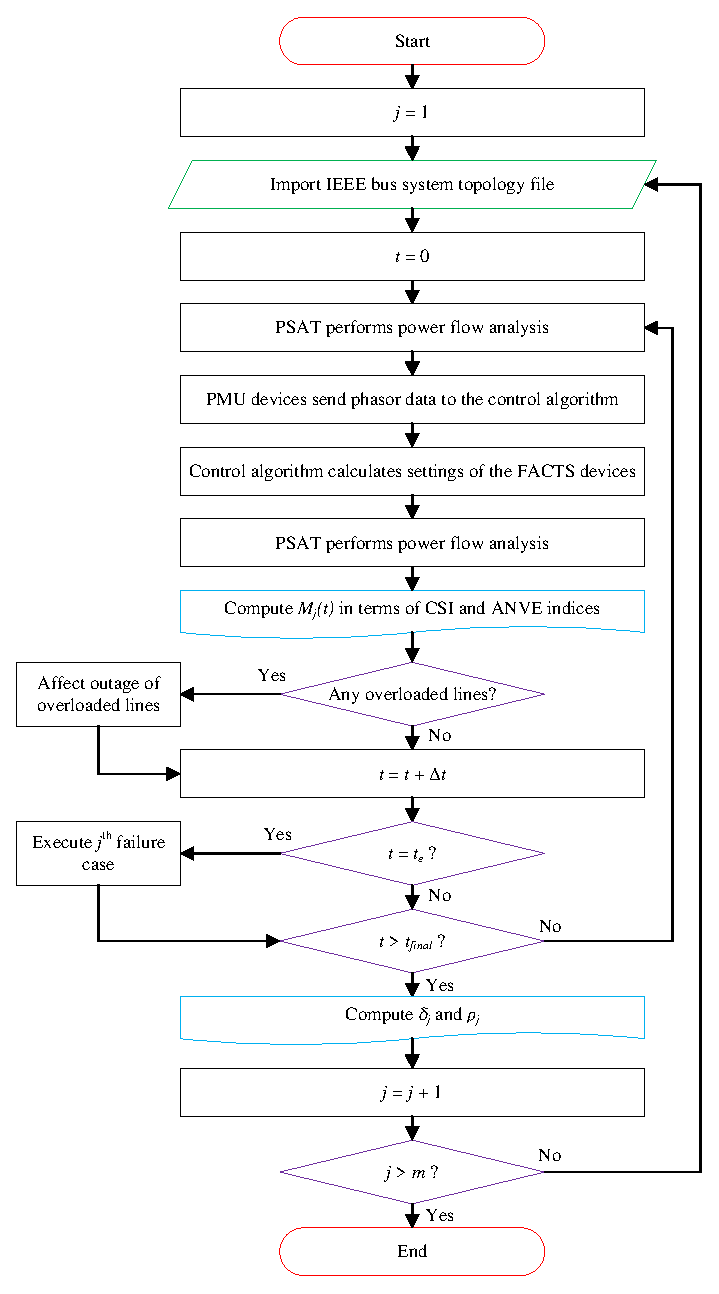
\includegraphics[width=0.70\columnwidth]{simulation_flowchart}
\caption{Survivability evaluation procedure.}
\label{fig:sim_flowchart}
\end{figure}

\subsection{Simulation Results}
\label{sec:case_study:results}
\figurename~\ref{fig:csi_anve_time} depicts the simulation results for each of the three test systems, using CSI and ANVE as the FoMs. In \figurename~\ref{fig:csi_anve_time}, each sub-figure depicts the change in one FoM over time, after the injection of a failure. The intensity of the line indicates the number of failure cases which the FoM demonstrated this behavior. Note that since the CSI is discrete, it can hold only a finite set of values between 0 and 1.

\begin{figure*}[!ht]
\centering
\subfloat[CSI vs. time for IEEE-14]
{\label{fig:csi_time_ieee14}
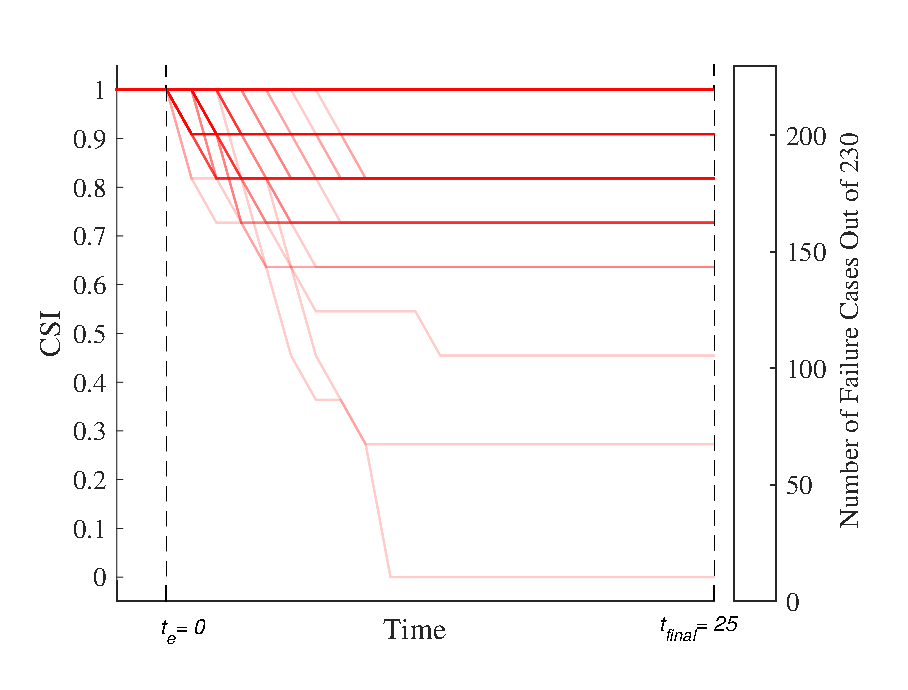
\includegraphics[width=0.32\linewidth]{ieee14_csi}}
\subfloat[CSI vs. time for IEEE-30]
{\label{fig:csi_time_ieee30}
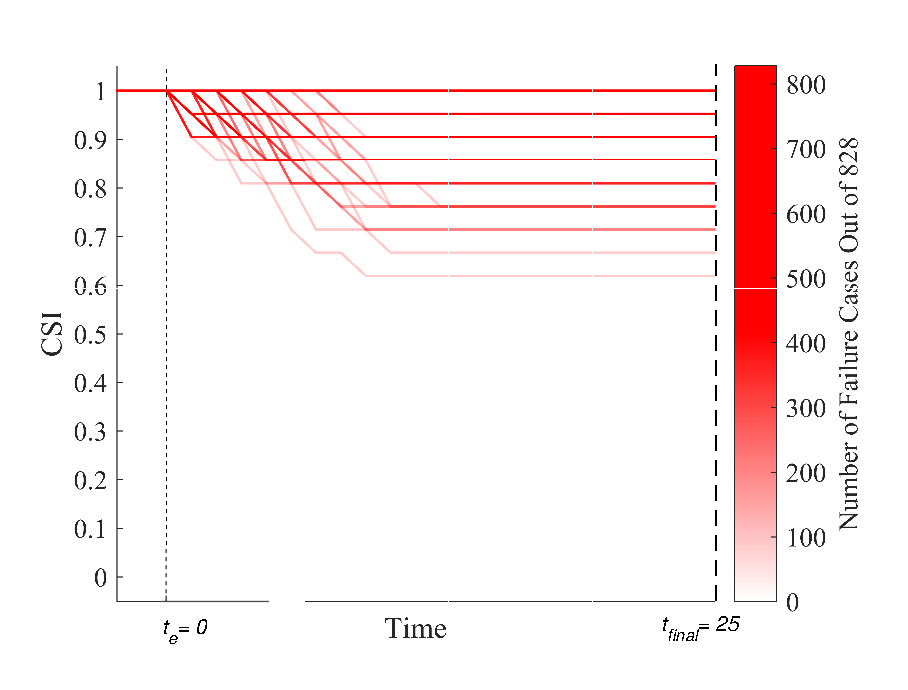
\includegraphics[width=0.32\linewidth]{ieee30_csi}}
\subfloat[CSI vs. time for IEEE-57]
{\label{fig:csi_time_ieee57}
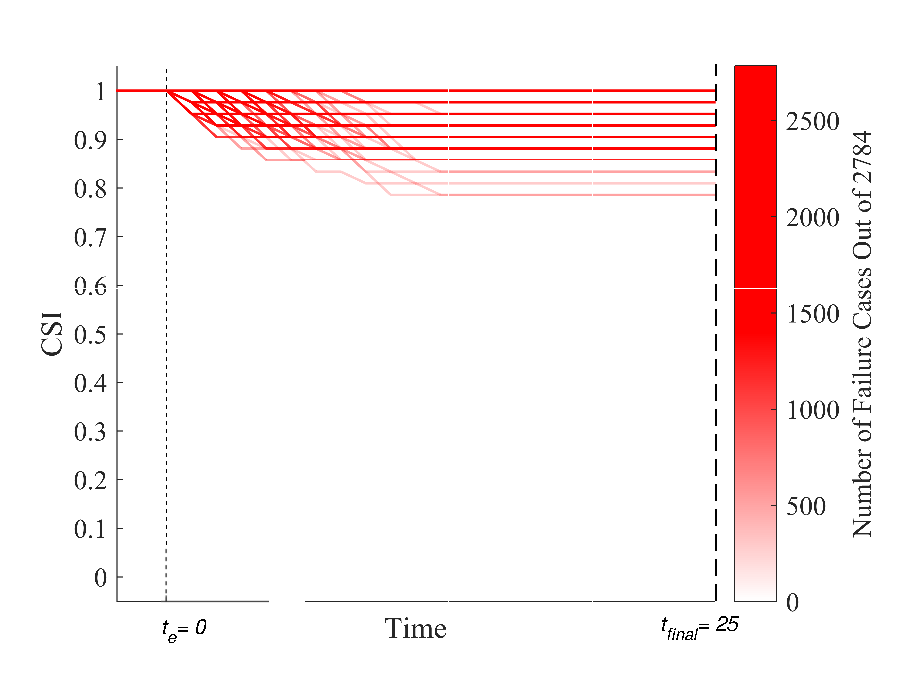
\includegraphics[width=0.32\linewidth]{ieee57_csi}}
\hfil
\subfloat[ANVE vs. time for IEEE-14]
{\label{fig:anve_time_ieee14}
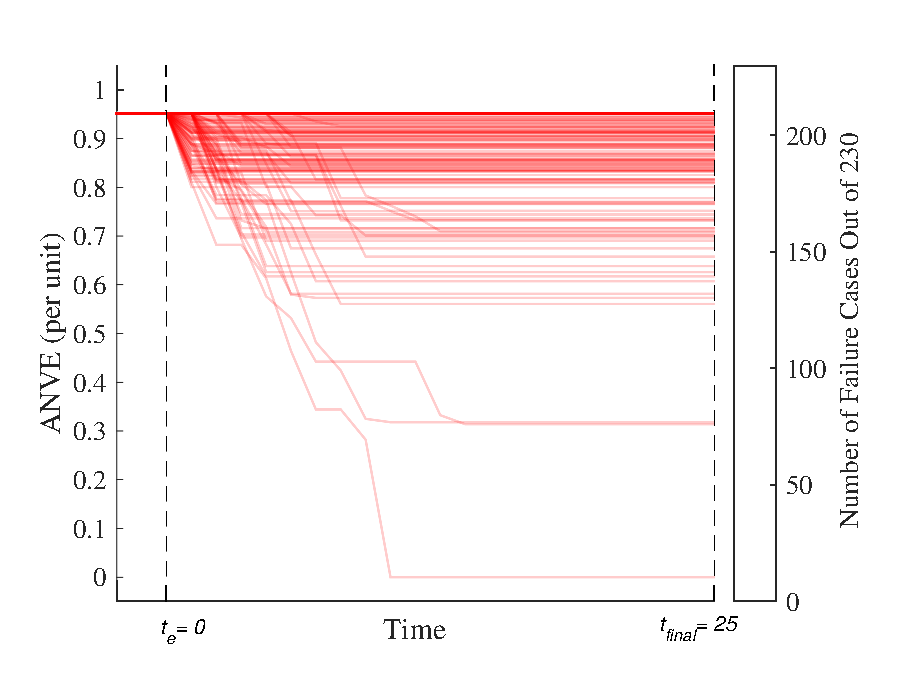
\includegraphics[width=0.32\linewidth]{ieee14_anve}}
\subfloat[ANVE vs. time for IEEE-30]
{\label{fig:anve_time_ieee30}
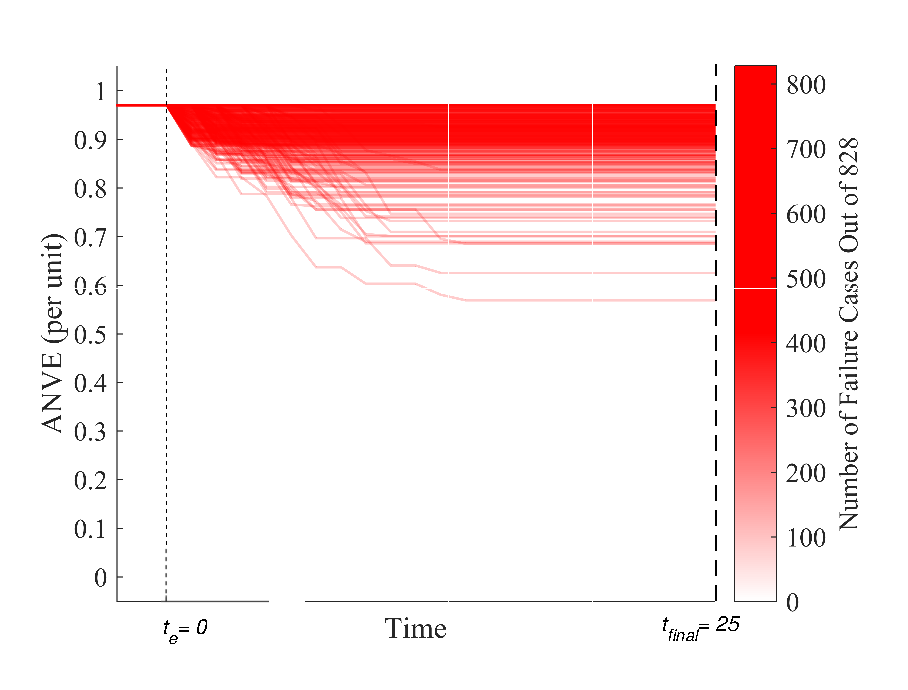
\includegraphics[width=0.32\linewidth]{ieee30_anve}}
\subfloat[ANVE vs. time for IEEE-57]
{\label{fig:anve_time_ieee57}
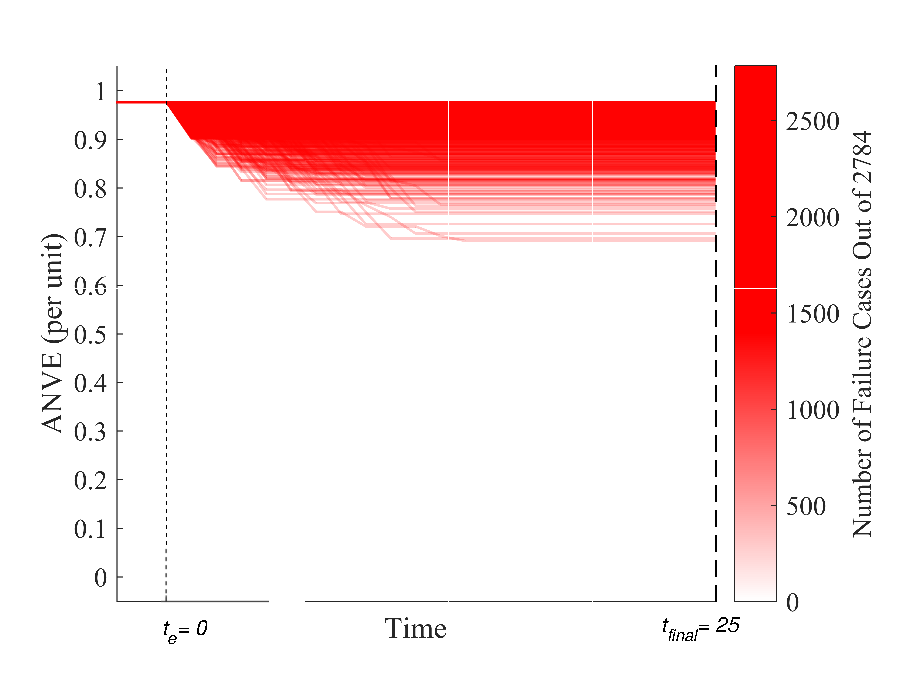
\includegraphics[width=0.32\linewidth]{ieee57_anve}}
\caption{CSI and ANVE vs. time. The desired outcome is a value of one for both CSI and ANVE, which indicates that all customers have been served, without voltage error.}
\label{fig:csi_anve_time}
\end{figure*}

These results indicate that minimal degradation is incurred in the majority of simulated failure cases. This is expected, given that the test systems are relatively robust. From the results for the IEEE-14 smart grid, shown in \figurename~\ref{fig:csi_time_ieee14} and \ref{fig:anve_time_ieee14}, it can be noted that a number of failures lead to total system failure - no customers served (CSI = 0) and maximum error (ANVE = 0). The IEEE-30 and 57 smart grids incorporate greater redundancy and can tolerate a greater number of failures. This robustness is reflected in \figurename~\ref{fig:csi_time_ieee30}, \ref{fig:anve_time_ieee30}, \ref{fig:csi_time_ieee57}, and \ref{fig:anve_time_ieee57}, where neither FoM reaches 0. Studies presented in~\cite{AlB17} and~\cite{SrE18} have reported similar standings of robustness of IEEE-14, IEEE-30, and IEEE-57, implying that the differences are due to the network topologies.

Also for a number of failure cases shown in \figurename~\ref{fig:csi_anve_time}, degradation of CSI and ANVE lags the disturbance by multiple time steps. By more careful inspection of these cases, it is observed that such behavior is correlated to cyber faults. For example, when a fault is injected to a PMU node, it remains dormant for multiple simulation time steps before causing a disruption in the physical system. Note that the FoM only captures the extent to which the physical service is provided and does not reveal the internal state of the cyber infrastructure. In practice, the duration of this propagation process is dependent on the architecture of the cyber network and can be instantaneous.

It is also seen in \figurename~\ref{fig:csi_anve_time} that a number of failure cases have two phases of system degradation separated by a brief period of stabilization. With further analysis, we observed that this behavior is correlated to propagation of faults to the cyber infrastructure during the disruption phase that later result in additional failures in the physical system. For example, power source of a PMU node is disconnected during the disruption phase, and in a few simulation time steps, lack of status data causes additional outages.

\subsection{Evaluation of Survivable Behavior}
\label{sec:case_study:surv_eval}
\figurename~\ref{fig:csi_anve_rate_extent_hist} depicts a two-dimensional histogram of CSI and ANVE for each smart grid simulated. These histograms are based on the maximum rate and extent of degradation calculated from the log of each failure case.

\begin{figure*}[!ht]
\centering
\subfloat[Extent vs. rate of CSI degradation for IEEE-14]
{\label{fig:csi_2dhist_ieee14}
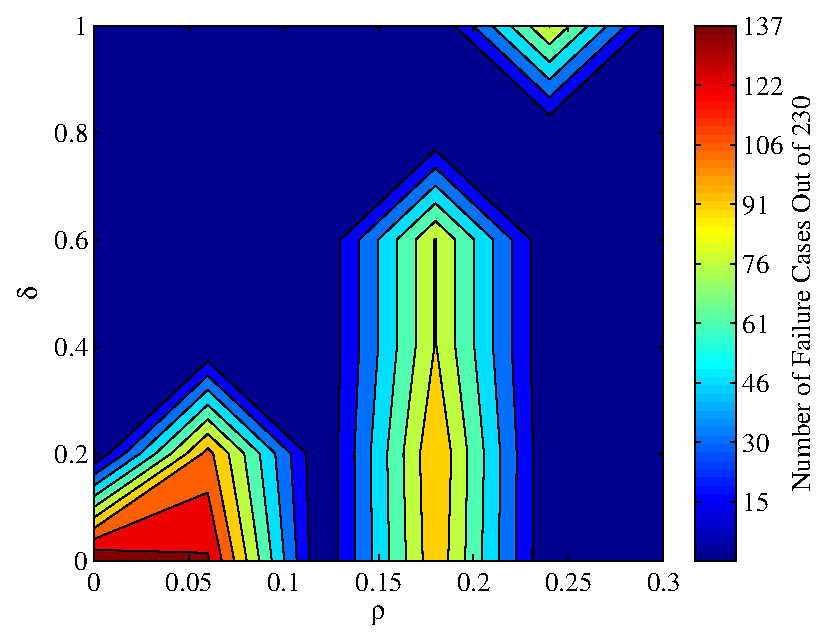
\includegraphics[width=0.32\linewidth]{ieee14_hist_csi}}
\subfloat[Extent vs. rate of CSI degradation for IEEE-30]
{\label{fig:csi_2dhist_ieee30}
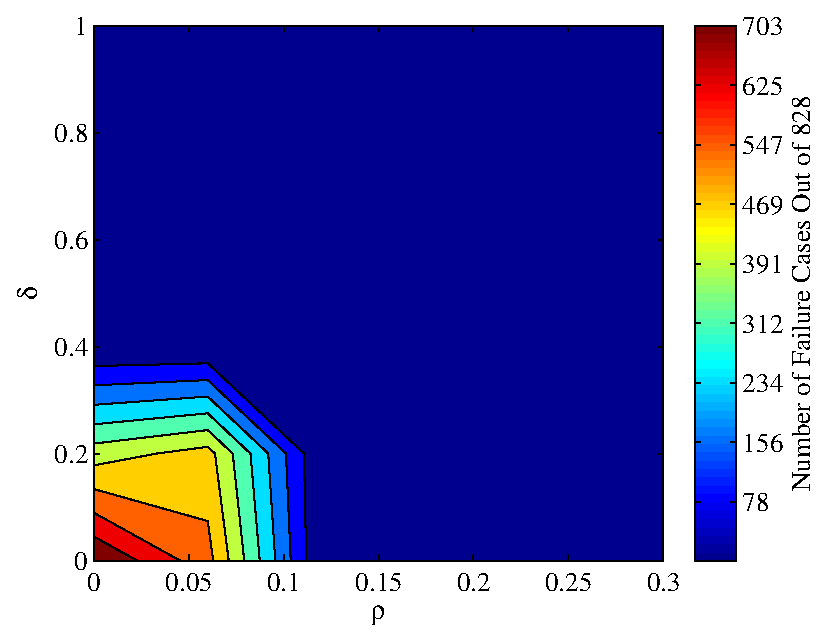
\includegraphics[width=0.32\linewidth]{ieee30_hist_csi}}
\subfloat[Extent vs. rate of CSI degradation for IEEE-57]
{\label{fig:csi_2dhist_ieee57}
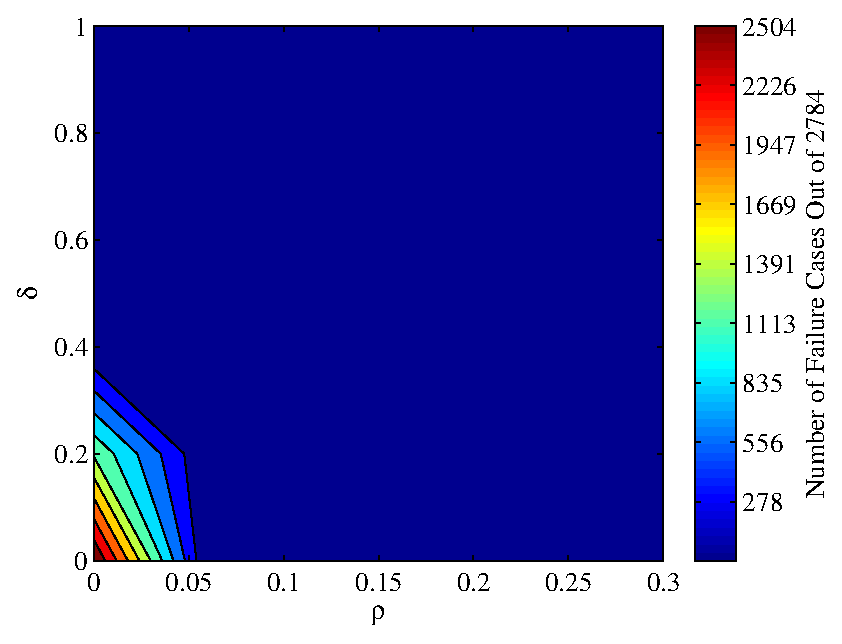
\includegraphics[width=0.32\linewidth]{ieee57_hist_csi}}
\hfil
\subfloat[Extent vs. rate of ANVE degradation for IEEE-14]
{\label{fig:anve_2dhist_ieee14}
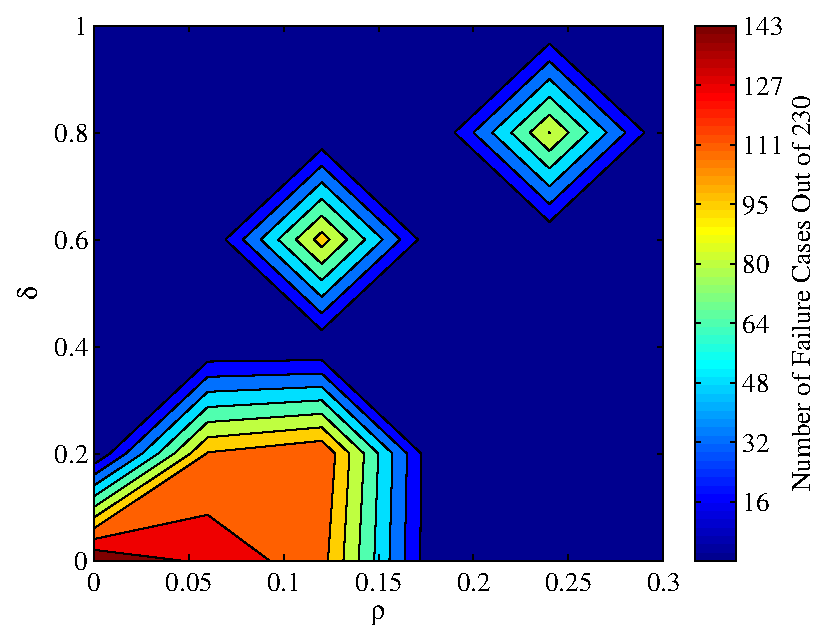
\includegraphics[width=0.32\linewidth]{ieee14_hist_anve}}
\subfloat[Extent vs. rate of ANVE degradation for IEEE-30]
{\label{fig:anve_2dhist_ieee30}
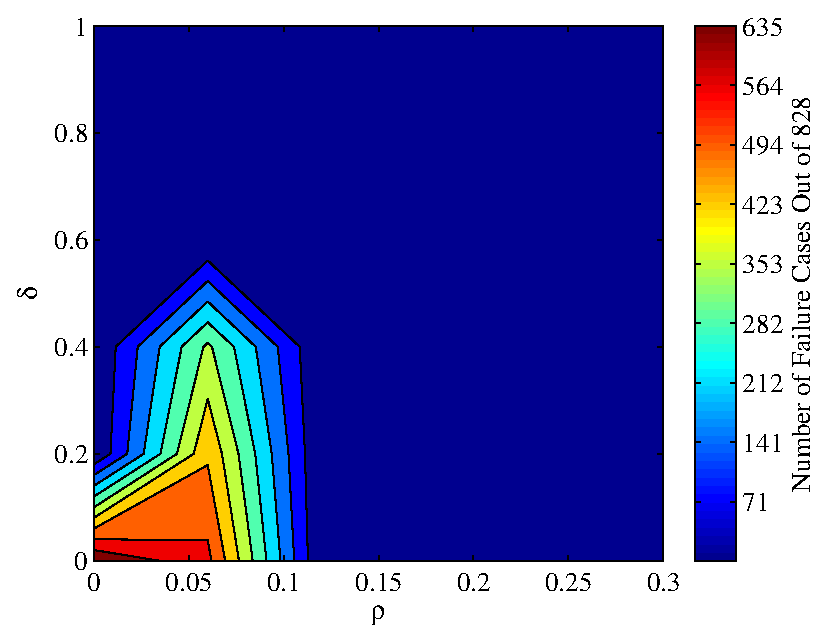
\includegraphics[width=0.32\linewidth]{ieee30_hist_anve}}
\subfloat[Extent vs. rate of ANVE degradation for IEEE-57]
{\label{fig:anve_2dhist_ieee57}
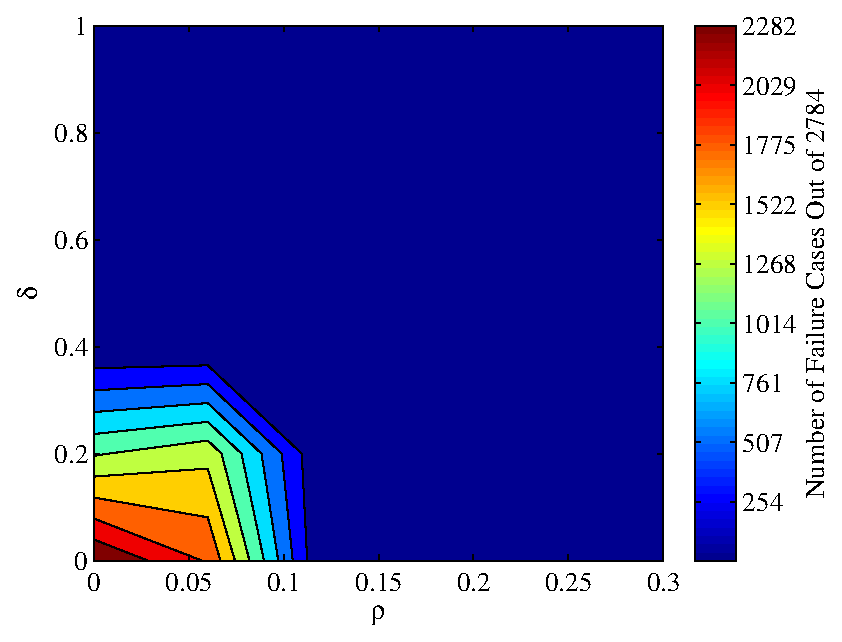
\includegraphics[width=0.32\linewidth]{ieee57_hist_anve}}
\caption{Histograms depicting the rate and extent of degradation of CSI and ANVE. The color indicates the number of failure cases for which the corresponding (rate, extent) pair was observed. For both CSI and ANVE, the desired outcome is a single cluster near the origin, reflecting slow and minimal degradation of the FoM.}
\label{fig:csi_anve_rate_extent_hist}
\end{figure*}

\figurename~\ref{fig:csi_anve_rate_extent_hist} gives better insight into the dynamics of the most critical failure cases and helps in identifying system's inabilities in executing failure resistance and/or graceful degradation. In an ideal system, every one of these histograms would be dense near the origin and sparse elsewhere, reflecting slow and minimal degradation in response to failure. This expectation is realized for the IEEE smart grids evaluated. However, there are clusters of failure cases with higher rates and extents of failure, which appear in the upper and/or right regions of the histogram. The presence of these clusters indicates that many of the failure cases simulated result in similar rates and extents of degradation. This is caused by similar failure propagation paths through the power grid, i.e., different cascading failures involving the same vulnerable components.

By further analysis of the failure cases that are reflected in the upper and/or right regions, we observe failure sequences that appear frequently towards the end of the simulation period. For example, in the case of IEEE 14-bus system, several of the failure cases that lead to severe degradation, end with the outage of the transmission line between bus 1 and bus 2 (denoted as $l_{1-2}$), followed by the outage of the transmission line between bus 1 and bus 5 (denoted as $l_{1-5}$). These two transmission lines act as bridges that connect the main generator, located at bus 1, to the load buses distributed in the network. Therefore, they typically operate at power flows that are close to their maximum limits. Disconnection of any alternative path of delivering power to the load buses can apply additional stress on these lines. If this additional stress leads to an overflow, $l_{1-2}$ and $l_{1-2}$ will trip and leave the system in a severely degraded or completely failed state.

Among the degradation points shown in the histograms of \figurename~\ref{fig:csi_anve_rate_extent_hist}, those that are not within an accepted distance from the origin should be inspected and resolved. In \figurename~\ref{fig:csi_2dhist_ieee14} and \ref{fig:anve_2dhist_ieee14}, there are multiple clusters that are associated with large ($\rho, \delta$) values, representing failure cases that result in sudden and/or severe loss of service. The information provided in these figures is instrumental in understanding the dynamics of the critical failures that we observed earlier in \figurename~\ref{fig:csi_time_ieee14} and \ref{fig:anve_time_ieee14}. Such information can also help in selecting best enhancement procedures. To resolve the limitations captured by clusters in the upper regions, i.e., system's inability in minimizing the extent of failures, additional redundancy and spatial separation is needed. For the example of IEEE-14, this can be attained by enhancing components involved in the critical failures. On the other hand, for addressing those clusters appeared in right regions, i.e., system's inability in degrading gracefully, real-time control strategies are required. For the example of IEEE-14, active reconfiguration schemes, such as intentional islanding, load shedding, and reciprocal altruism are shown to be efficient~\cite{PaY13}.

\subsection{Importance Analysis}
\label{sec:case_study:import_analysis}
In importance analysis, we seek to identify bottlenecks to survivability and guide investments in fortifying a system. To this end, criticality and fragility can be used as measures of the importance of a component, as described in Section~\ref{sec:approach:importance}.

Table~\ref{tab:weakness} lists the top ten lines of the IEEE 57-bus smart grid, ranked by fragility and criticality, respectively. It can be seen that some lines rank similarly by both measures, e.g., lines $l_{4-18}$, $l_{3-4}$, and $l_{4-6}$. In contrast, a few lines, such as $l_{8-9}$ and $l_{6-7}$, are far more critical than they are fragile, i.e., these lines fail in a relatively small fraction of failure cases, but when they do fail, they cause significant degradation of the system FoM. Conversely, a few lines, such as $l_{1-2}$ and $l_{1-15}$, can be considered fragile, but non-critical. These lines fail when a more important line fails, but their failure is relatively insignificant in terms of system survivability.

\begin{table}[t!]
\centering
\caption{Transmission lines of IEEE 57-bus system, ranked by fragility and criticality, respectively. Only the top ten lines are shown.}
\label{tab:weakness}
\renewcommand{\arraystretch}{1.1}
\renewcommand\tabcolsep{4pt}
\begin{tabular}{ccc|ccc}
  \textbf{Rank} & \textbf{Line} & \textbf{Fragility} \scriptsize($\times 10$) & \textbf{Rank} & \textbf{Line} & \textbf{Criticality} \scriptsize($\times 10^2$)\\
\hline
	1  & $l_{4-18}$ & 0.2801 & 1  & $l_{8-9}$   & 0.1477 \\
	2  & $l_{1-2}$  & 0.2729 & 2  & $l_{4-18}$  & 0.1417 \\
	3  & $l_{3-4}$  & 0.2514 & 3  & $l_{3-4}$   & 0.1337 \\
	4  & $l_{1-15}$ & 0.2370 & 4  & $l_{6-7}$   & 0.1277 \\
	5  & $l_{1-17}$ & 0.2370 & 5  & $l_{4-6}$   & 0.1137 \\
\hline
	6  & $l_{4-6}$  & 0.2227 & 6  & $l_{1-2}$   & 0.1078 \\
	7  & $l_{8-9}$  & 0.2227 & 7  & $l_{1-15}$  & 0.1058 \\
	8  & $l_{1-16}$ & 0.2227 & 8  & $l_{13-15}$ & 0.0718 \\
	9  & $l_{6-7}$  & 0.2155 & 9  & $l_{1-16}$  & 0.0659 \\
	10 & $l_{2-3}$  & 0.1939 & 10 & $l_{2-3}$   & 0.0639 \\
\end{tabular}
\end{table}

\subsection{Validation of Approach}
In this section we validate our importance analysis technique through targeted hardening of a IEEE 57-bus smart grid. The hardening effort involves fortifying each of the five most important transmission lines, by increasing their power flow capacity by 50\%. This is expected to increase the survivability of the system, as it increases fault tolerance. The same hardening effect could have been achieved by adding redundant lines; however, this alternative was eliminated to maintain the topology of the system for ease of comparison. Survivability analysis was carried out for each hardened grid, to determine whether the hardening improved survivability. For the sake of brevity, we have only presented results based on CSI, however improvements are confirmed based on ANVE too.

\begin{figure}[!ht]
\centering
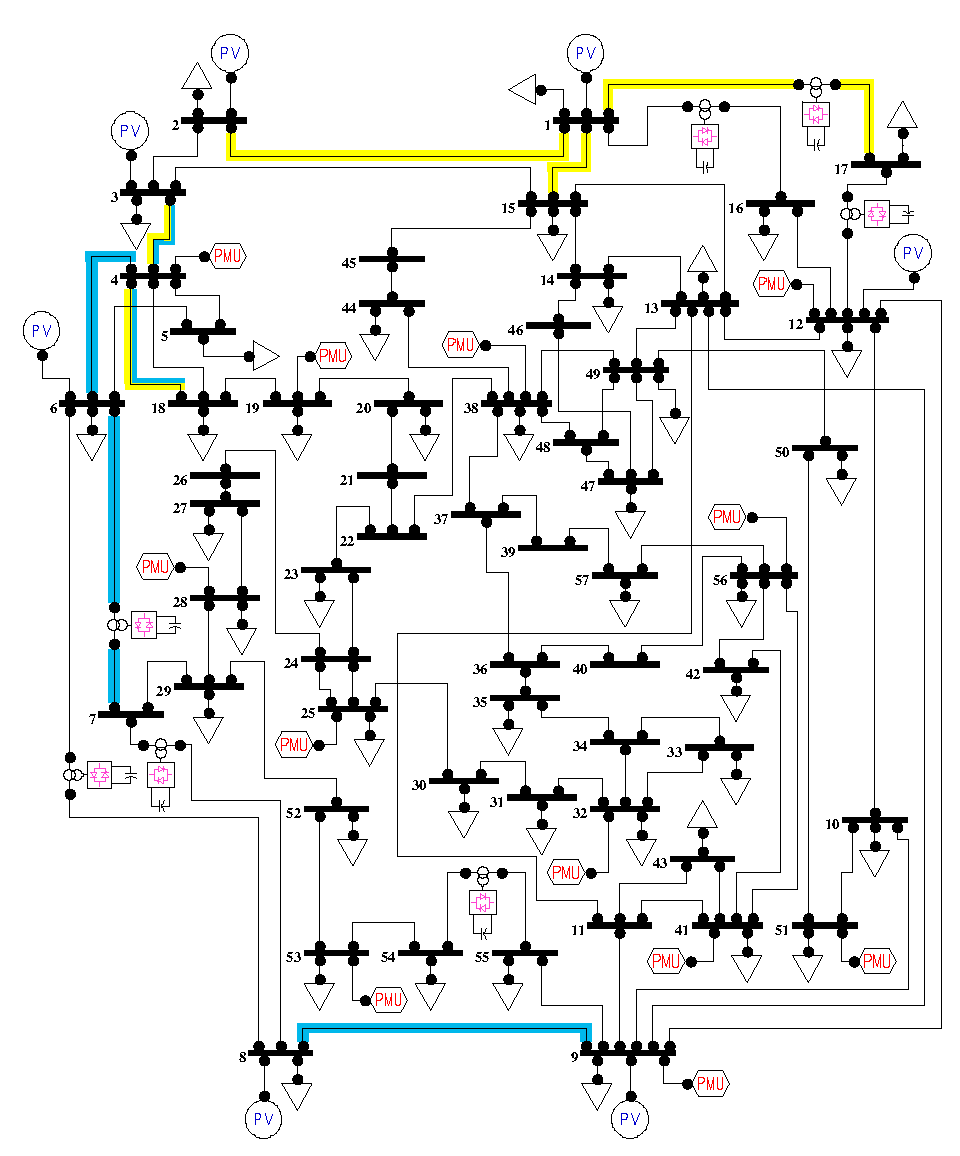
\includegraphics[width=0.95\columnwidth]{ieee57_highlighted}
\caption{IEEE 57-bus smart grid test system. Most fragile lines are highlighted in yellow. Most critical lines are highlighted in blue.}
\label{fig:ieee57_highlighted}
\end{figure}

The first set of hardening efforts used fragility as a measure of importance. The lines chosen for hardening, $l_{4-18}$, $l_{1-2}$, $l_{3-4}$, $l_{1-15}$, and $l_{1-17}$, are highlighted in yellow in \figurename~\ref{fig:ieee57_highlighted}. Criticality was subsequently used to select components for hardening. Lines $l_{8-9}$, $l_{4-18}$, $l_{3-4}$, $l_{6-7}$, and $l_{4-6}$, shown highlighted in blue in \figurename~\ref{fig:ieee57_highlighted}, were hardened. The CSI of the original IEEE 57-bus smart grid and each of its hardened versions are shown in \figurename~\ref{fig:ieee57_csi_comp}. The corresponding survivability histograms appear in \figurename~\ref{fig:ieee57_hist_csi_comp}. While both of the hardened systems attain higher survivability than the original system, the improvements of the hardening based on criticality are more significant. This is expected considering the fact that criticality is a more precise metric than fragility.

\begin{figure*}[!ht]
\centering
\subfloat[CSI vs. time for original IEEE-57]
{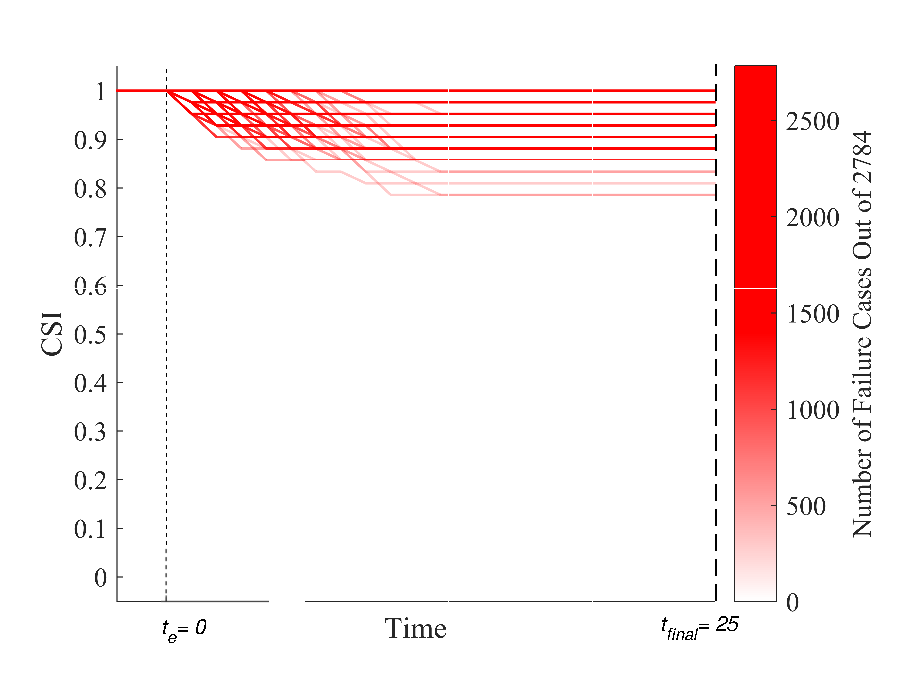
\includegraphics[width=0.32\linewidth]{ieee57_csi}
\label{fig:ieee57_csi_orig}}
\subfloat[CSI vs. time for IEEE-57 hardened based on fragility]
{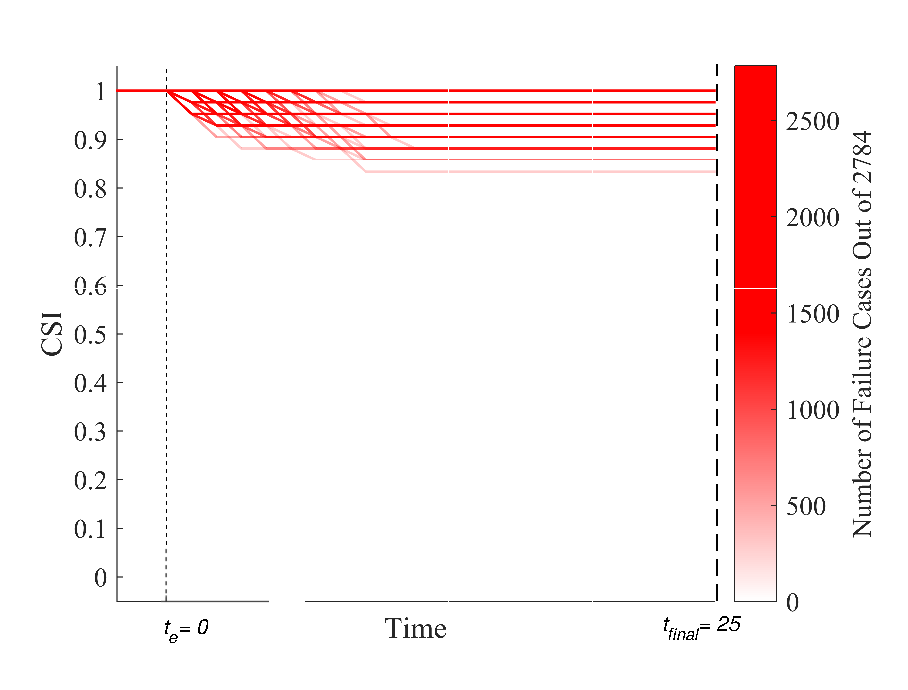
\includegraphics[width=0.32\linewidth]{ieee57_csi_hardened_frag}
\label{fig:ieee57_csi_hardened_frag}}
\subfloat[CSI vs. time for IEEE-57 hardened based on criticality]
{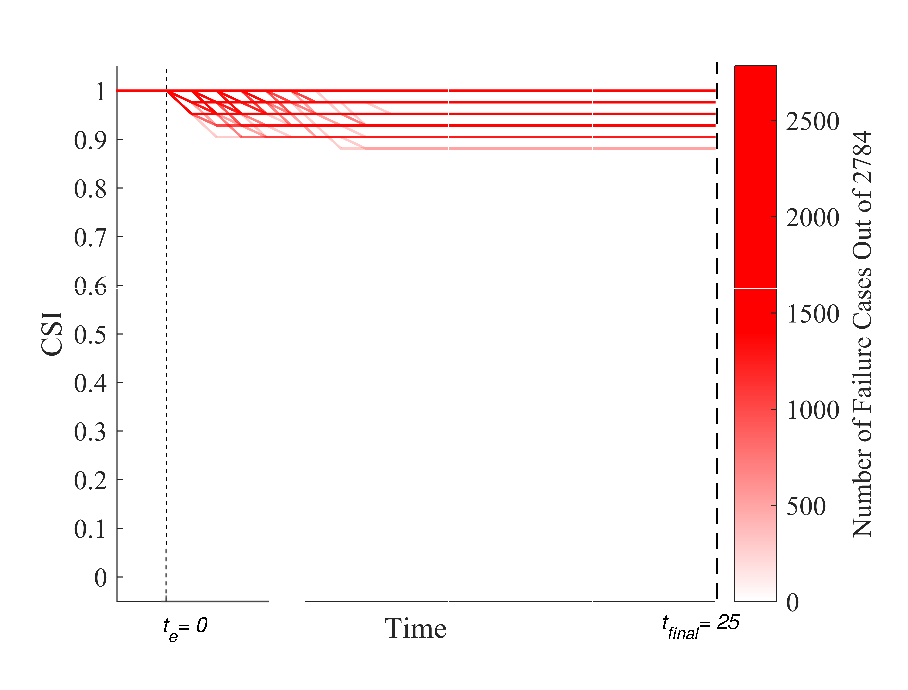
\includegraphics[width=0.32\linewidth]{ieee57_csi_hardened_crit}
\label{fig:ieee57_csi_hardened_crit}}
\caption{Comparison of CSI for original and hardened IEEE-57. Hardening based on either importance measure has reduced the extent of degradation.}
\label{fig:ieee57_csi_comp}
\end{figure*}

\begin{figure*}[!ht]
\centering
\subfloat[Extent vs. rate of CSI degradation for original IEEE-57]
{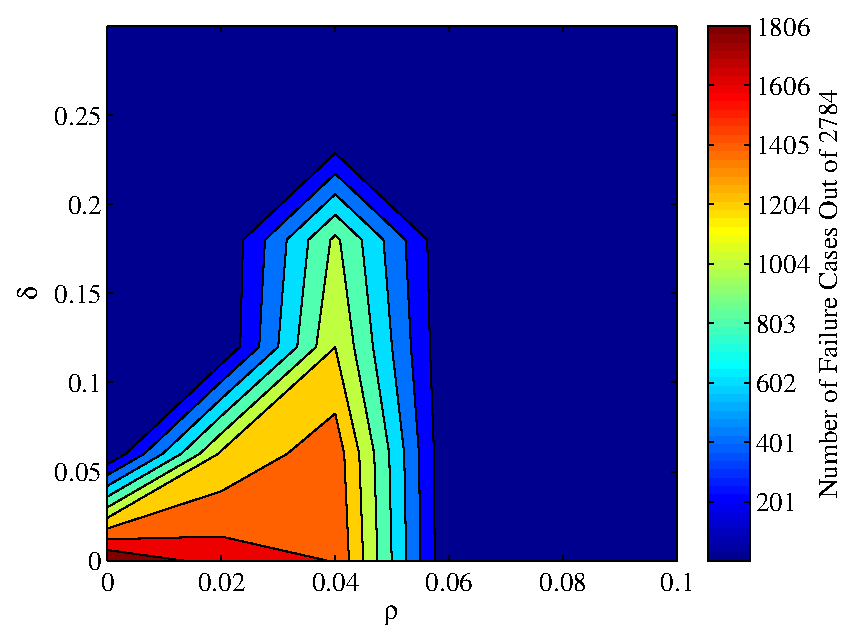
\includegraphics[width=0.32\linewidth]{ieee57_hist_csi_zoomed}
\label{fig:ieee57_hist_csi_orig}}
\subfloat[Extent vs. rate of CSI degradation for IEEE-57 hardened based on fragility]
{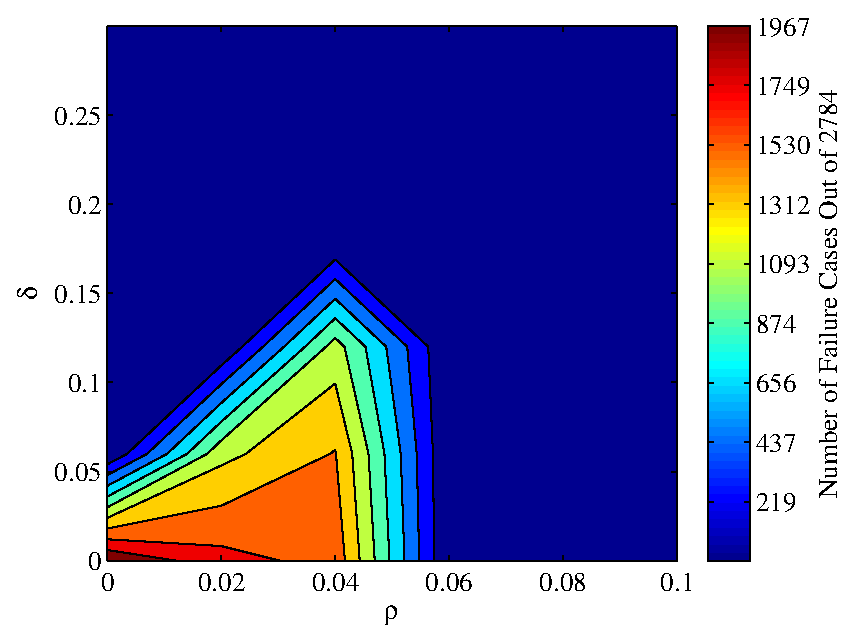
\includegraphics[width=0.32\linewidth]{ieee57_hist_csi_hardened_frag}
\label{fig:ieee57_hist_csi_hardened_frag}}
\subfloat[Extent vs. rate of CSI degradation for IEEE-57 hardened based on criticality]
{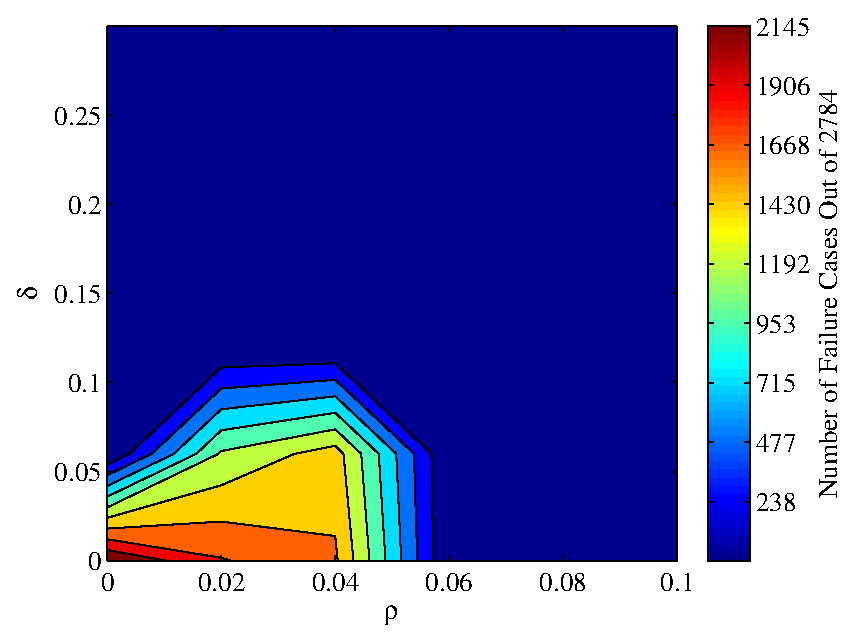
\includegraphics[width=0.32\linewidth]{ieee57_hist_csi_hardened_crit}
\label{fig:ieee57_hist_csi_hardened_crit}}
\caption{Comparison of histograms depicting the rate and extent of degradation of CSI for original and hardened IEEE-57. Clusters of degradation points have moved towards the origin for both hardened systems.}
\label{fig:ieee57_hist_csi_comp}
\end{figure*}

Note that the improvements observed in \figurename~\ref{fig:ieee57_hist_csi_comp} are mostly towards movement of the clusters in the upper regions of the histogram to the bottom, i.e., limiting the extent of degradation, while no significant changes are observed in the horizontal direction, i.e., limiting the rate of degradation. This is expected since the enhancements have been applied only in the form of increased power capacity. For changing the temporal dynamics of the system in response to failures, active reconfiguration schemes need to be devised and employed. In this work, we have not analyzed such mechanisms, but several studies have reported applicability of these techniques in power grids~\cite{PaY13}.

\section{Conclusion}
\label{sec:conc}
We have presented an approach for evaluation of survivability for cyber-physical smart grids with arbitrary, yet known topologies. Our approach is based on observation or simulation of multiple failure cases for the system. For each failure case, we determine the rate and extent of degradation of a domain-specific FoM chosen to represent the provision of an essential service by the system. We have demonstrated the use of this information in importance analysis, where the goal is to identify critical components whose hardening would be most beneficial to survivability. We illustrated the application of this technique to three smart grid networks based on conventional IEEE test systems.

In future work, we plan to:
\begin{enumerate}
  \item refine our evaluation of survivability by using a multi-dimensional FoM and its Pareto optima,
  \item improve the scalability of our approach through more strategic selection of failure cases and investigate the use of superposition for evaluating the survivability of systems with independent components,
  \item study methods for identification and elimination of failure cases with similar failure sequences and common failure propagation paths,
  \item apply the proposed method to other CPSs, and
  \item study applicability of FoM abstraction in quantitative modeling of safety and security aspects of a system.
\end{enumerate}

\section*{Acknowledgments}
We gratefully acknowledge support from the US Departments of Transportation and Education, the National Science Foundation, and the Center for Infrastructure Engineering Studies and Intelligent Systems Center at the Missouri University of Science and Technology.

\bibliography{final_abbrv}

\end{document}
